\newpage
\section{Results}

This section presents the results and their respective conclusion on all the experiments and their preliminary tests.

\subsection{Girvan-Newman approximation}


\textbf{Preliminary test}

The results of the semi-supervised classification task on the CORA dataset are show on the following table:


\begin{table}[H]
\centering
\begin{tabular}{|llccc|c}
%\toprule
\hline
    Model &           params &   Val Loss &   Test Accuracy &   Duration \\
%\midrule
\hline
   SGConv &   100\_epochs=200 &     1.7587 &   0.790 ± 0.018 &      0.585 \\
 ChebConv &   100\_epochs=200 &     0.8133 &   0.769 ± 0.027 &      5.049 \\
    APPNP &   100\_epochs=200 &     0.8894 &   0.808 ± 0.017 &      0.984 \\
  GATConv &   100\_epochs=200 &     0.8111 &   0.803 ± 0.016 &      1.967 \\
  GCNConv &   100\_epochs=200 &     0.8864 &   0.789 ± 0.018 &      1.091 \\
%\bottomrule
\hline
\end{tabular}
\label{preliminar_GN}\caption{Reproduced benchmark semi-supervised classification experiments on CORA dataset }
\end{table}

We observe that test accuracy is correct in all the models trained, successfully replicating the experiments. Setup of the environment is also correctly verified.




\textbf{Main experiment}

As detailed in the experiments section, the main experiment is to train a model to approximate the edge betweenness of part of the edges of a graph, in a semi-supervised manner. The results,  measured with the accuracy after transforming the edge betweenness values into a finite number of ranges (bucketization or discretization), are shown in the folling table:

\begin{table}[H]
\centering
\begin{tabular}{|llllccc|}
\hline
 Model &                                                                        Paramteres  &  Runs\/Epochs  &  Splits &    Loss &        Accuracy &  Time(min) \\
\hline
 META1 &          d19d16h10e19n16n15 & 1-2 & 20-500-1500 &  1.6367 &     0.239  &      0.069 \\
 META2 &       d19d16h10e19n16n15 & 100-20 & 20-500-1500 &  1.7550 &   0.296 ± 0.031 &      0.494 \\
 META3 &      d19d16h10e19n16n15 & 100-200 & 20-500-1500 &  2.7132 &   0.274 ± 0.019 &      3.518 \\
 META4 &      d19d16h10e19n16n15 & 100-20 & 20-500-10556 &  1.7508 &   0.293 ± 0.023 &      0.547 \\
 META5 &     d19d16h10e19n16n15 & 100-200 & 20-500-10556 &  2.8676 &   0.266 ± 0.013 &      3.743 \\
 META6 &     d19d16h10e19n16n15 & 100-20 & 20-4000-10556 &  1.7437 &   0.296 ± 0.026 &      0.528 \\
 META7 &    d19d16h10e19n16n15 & 100-200 & 20-4000-10556 &  2.8105 &   0.265 ± 0.016 &      3.704 \\
 META8 &    d19d16h10e19n16n15 & 100-20 & 300-4000-10556 &  1.1625 &   \textbf{0.563 ± 0.067} &      0.506 \\
 META9 &   d19d16h10e19n16n15 & 100-200 & 300-4000-10556 &  2.3160 &   0.409 ± 0.033 &      3.546 \\
 META10 &    d10d10h10e10n10n10 & 100-20 & 300-4000-10556 &  1.1565 &   0.537 ± 0.074 &      0.494 \\
 META11 &   d10d10h10e10n10n10 & 100-200 & 300-4000-10556 &  2.1036 &   0.374 ± 0.030 &      3.593 \\
\hline
\end{tabular}
\label{Experiment1}\caption{Edge betweenness approximation with a graph neural network experiment}
\end{table}

The maximum accuracy obtained is 56.3\% (out of 5 classes) by the model META8. The following plots show the distribution of predicted values compared to the real values, both for the discrete and real values.





\begin{figure}[H]
\minipage{0.5\textwidth}%
  \centering
    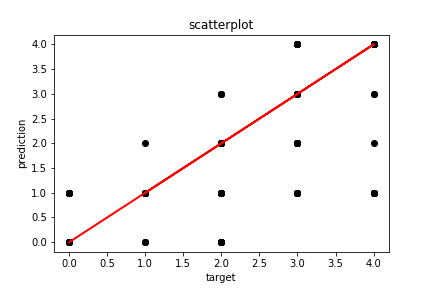
\includegraphics[width=0.9\linewidth]{img/GN_exp1/2019-09-28_22-02-07_META1_d4=19_d5=16_hus=10_eus=19_n1us=16_n2us=15_r=100_epochs=20_split-300-4000-10556-_scatterplot.png}
\endminipage
\minipage{0.5\textwidth}%
  \centering
    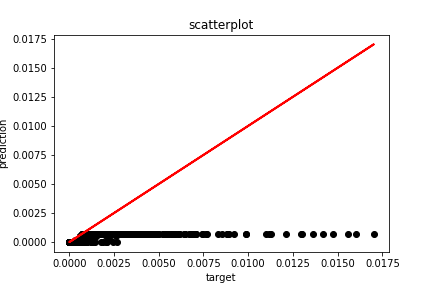
\includegraphics[width=0.9\linewidth]{img/GN_exp1/2019-09-28_22-02-07_META1_d4=19_d5=16_hus=10_eus=19_n1us=16_n2us=15_r=100_epochs=20_split-300-4000-10556-_scatterplot_real_eb.png}
\endminipage
\caption{Scatter plot comparing target edge betweenness and predicted (discrete range and real values)}\label{fig:edgeb_exp1_scatter}
\end{figure}


\begin{figure}[H]
\minipage{0.5\textwidth}%
  \centering
    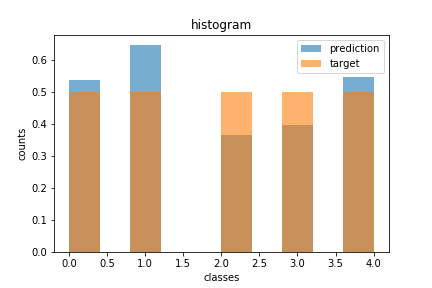
\includegraphics[width=0.9\linewidth]{img/GN_exp1/2019-09-28_22-02-08_META1_d4=19_d5=16_hus=10_eus=19_n1us=16_n2us=15_r=100_epochs=20_split-300-4000-10556-_histogram.png}
\endminipage
\minipage{0.5\textwidth}%
  \centering
    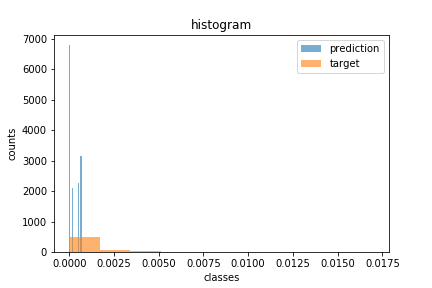
\includegraphics[width=0.9\linewidth]{img/GN_exp1/2019-09-28_22-02-08_META1_d4=19_d5=16_hus=10_eus=19_n1us=16_n2us=15_r=100_epochs=20_split-300-4000-10556-_histogram_real_eb.png}
\endminipage
\caption{histogram of target values versus predicted values of edge betweenness in both discrete and continuous display }\label{fig:edgeb_exp1_histogra}
\end{figure}



\begin{figure}[H]
\minipage{0.5\textwidth}%
  \centering
    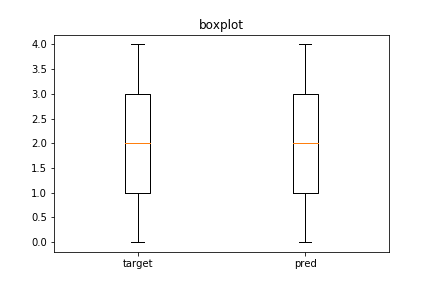
\includegraphics[width=0.9\linewidth]{img/GN_exp1/2019-09-28_22-02-08_META1_d4=19_d5=16_hus=10_eus=19_n1us=16_n2us=15_r=100_epochs=20_split-300-4000-10556-_boxplot.png}
\endminipage
\minipage{0.5\textwidth}%
  \centering
    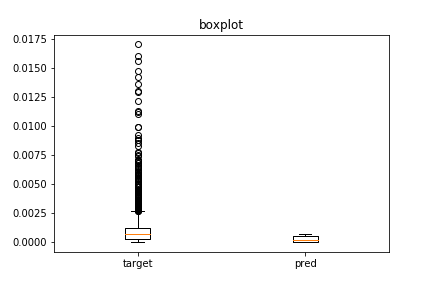
\includegraphics[width=0.9\linewidth]{img/GN_exp1/2019-09-28_22-02-08_META1_d4=19_d5=16_hus=10_eus=19_n1us=16_n2us=15_r=100_epochs=20_split-300-4000-10556-_boxplot_real_eb.png}
\endminipage
\caption{Boxplot of target values versus predicted values of edge betweenness in both discrete and continuous display }\label{fig:edgeb_exp1_boxplot}
\end{figure}



\textbf{Conclusion}
% conclusion on results

% value the results, how good is this accuracy vs random model
The trained model for predicting the edge betweenness obtains a 56.3\% accuracy on a 5 classes classification model(edge betweenness real values are grouped into buckets that conform the set of classes). A random classifier would have a 20\% accuracy if classes where balanced. We can conclude that the model is not bad as it obtains a 36.3\% uplift on accuracy versus a random model.
% problems that this model could exhibit: higher range has more variability than others, which for finding the maximum value is problematic.
One important negative aspect of the models trained so far in this experiment, is that the predictive model will not predict which edge has maximum value of edge betweenness but a whole group or bucket. The final goal of the experiment is to use the model for the Girvan-Newman algorithm which needs to find the edge with highest edge betweenness. Since the model uses buckets, all edge betweennesses predicted to belong to a bucket will have all the same value. The results presented used the minimum value of the bucket, to help accuracy.

\textbf{Improvements}
% Improvements.

The first basic improvement that could be looked into is to perform a longer hyper parameter (and data partitioning configuration) search, to see if this kind of model can obtain a better accuracy. It could also be trained on a larger set of buckets or classes. 


Also, it would be important to test its performance on several heterogeneous graphs, to get an idea of how stable this model training is.


%higher values for the Girvan Newman
To improve the usability for the Girvan-Newman approximation, the precision in high values should be increased. One naïve solution would be to give the samples in the bucket their maximum value, because the problem is to find the real maximum and not to increase the overall values of a bucket. In one hand, to have the model to predict higher values, a smaller range with the most higher values of the training set could be created. But, since this would introduce a great deal of class imbalance, the performance of the model would decrease. This trade-off should be tested thoroughly. A good approach to solve the class imbalance would be to used a weighted loss function during the training of the Graph Neural Network. This loss would have a weight associated with the inverse of the number of samples a bucket contains. Another thing to keep in mind, is that the loss function and the error function(metric score) should be changed to something more beneficial for finding the maximal values. One different approach to this problem would be to recompute the real edge betweenness of edge predicted to belong to the highest bucket. Depending on the size of the higher bucket, this process could harm the speed of the algorithm.

Finally, for the Girvan-Newman algorithm, an inductive setup of the graph neural network algorithm should be tested.  The current transductive setup (semi-supervised learning where a few edge betweennesses will be actually computed to quickly train the model and the rest will be predicted) might impact the speed of execution. Since in each iteration some edge betweenness need to be computed, then the model needs to be trained (or fine-tuned) and then this same model is used to predict the rest of edge betweenness's, the process could be slower than the original algorithm. If a model is trained once and can directly be used in each iteration, the overall process should be faster. There is a middle ground solution, where the graph neural network model is only trained in the very first iteration of the Girvan-Newman algorithm and then in the subsequent steps it is just used for prediction. 




% 2) Function Renaming:
% results table: noisy dataset:   models | cv score | test score macro avg
% results table: v1 dataset:   models | cv score | test score macro avg
% results table: v2 dataset:   models | cv score | test score macro avg
% results table: v3 dataset:   models | cv score | test score macro avg

% conclusion on results



% idea: polyorphism on code, hacking the art of exploitation chap5, even with xor or sub, a code can be rewritten => STRUCTURE IS NOT KEY TO FUNCTIONALITY ON CODE (but still I was hoping on some similar structure coming from similar compilers/programing languages/SO interfaces..)
